\chapter{Introduction}\label{ch:Introduction}

\section{Intro}
    \discuss{feel free to provide insights, everything here is up for alteration, and this section will change during the project--- I'm pretty much just pulling it out of my butt at this point}
    
    - the daily life of people with a lack of limbs is filled with hardship, and inconveniences, \\
    - in order to improve their life more advanced prostheses are needed\\
    - in today's welfare society, we try to improve the living standard of all. we know that not all are living with the same possibilities as others and as such we strive to improve the life's of others. 
    one group with more obstacles in life than most is the amputees, people who have for some reason lost part of themselves\\
    
\textbf{intro}. in today's world, people try to life to the best of their ability. we try to improve our lives with material goods, and continue to seek more and better accessories. but for some these goods have a whole other meaning. for some its a part of them selves
in this report we will investigate the problems involved in improving the lives of people suffering from loss of limbs. with a specific focus on high level arm amputations. 
we will investigate the use of robotics in prostheses, how these can help in the daily life of people and when a robotic solution is a better option for the individual than a conventional rigid option.

this report will focus on the creation of a robotic arm prostheses, and investigating the hardships involved in its creation. 


\textbf{The end user}
We will focus on 
users having Shoulder disarticulation

\textbf{the social benefits}

\textbf{conventional prostheses}

\textbf{Who are we}
We are a study-group located in Aalborg Denmark, we are third semester robotics students

\textbf{we will overlook}

\textbf{Goal}
In this project we will work towards using a minimal amount of muscles to manipulate a robotic arm to do a given task

    
    
    
\section{Initial Problem Formulation}

How can a person with a Shoulder disarticulation(upper limb amputees), with focus on a robotic prostheses.
\begin{itemize}
    \item What kind of robotic prosthesis would be best suited to assist a person with a shoulder disarticulation.
    \item What control method would be relevant for a user suffering from shoulder disarticulation.
    \item What safety measures are needed to insure the end-user safety.
\end{itemize}
\paragraph{explanatory text}


\section{Stakeholder Analysis}
The project is structured with the use of an stakeholder analysis in order to find the groups that effects or is affected by the project.
First, the different groups are found by brainstorming and then sorted into a power/interest matrix. \\
\subsection{Power/Interest Matrix}
The power/interest matrix sorts the different groups into four categories, which assures that the project considers the groups that are most important. At the same time, the matrix illustrates the relationship between the different groups of stakeholders along with an assessment of importance. 
\begin{define}{Power and Interest}
This project define the stakeholders power as the stakeholders ability to influence the project, and the stakeholders interest as the degree of which the project influence the stakeholder. 
\end{define}
\begin{figure}[H]
    \centering
    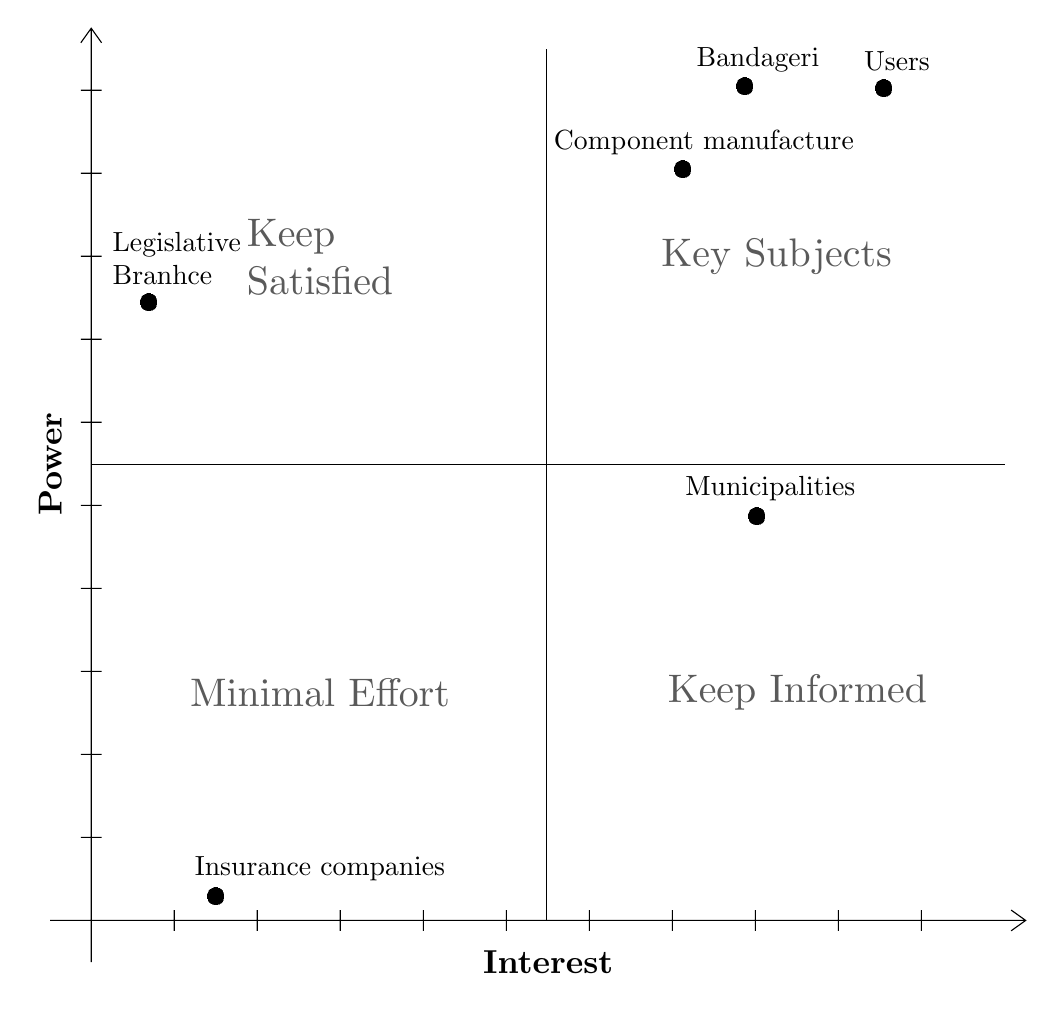
\begin{tikzpicture}[x=0.75pt,y=0.75pt,yscale=-1,xscale=1]
%uncomment if require: \path (0,488.142858505249); %set diagram left start at 0, and has height of 488.142858505249

%Shape: Axis 2D
\draw  (20,429.86) -- (490,429.86)(39.79,0) -- (39.79,450) (483,424.86) -- (490,429.86) -- (483,434.86) (34.79,7) -- (39.79,0) -- (44.79,7) (79.79,424.86) -- (79.79,434.86)(119.79,424.86) -- (119.79,434.86)(159.79,424.86) -- (159.79,434.86)(199.79,424.86) -- (199.79,434.86)(239.79,424.86) -- (239.79,434.86)(279.79,424.86) -- (279.79,434.86)(319.79,424.86) -- (319.79,434.86)(359.79,424.86) -- (359.79,434.86)(399.79,424.86) -- (399.79,434.86)(439.79,424.86) -- (439.79,434.86)(34.79,389.86) -- (44.79,389.86)(34.79,349.86) -- (44.79,349.86)(34.79,309.86) -- (44.79,309.86)(34.79,269.86) -- (44.79,269.86)(34.79,229.86) -- (44.79,229.86)(34.79,189.86) -- (44.79,189.86)(34.79,149.86) -- (44.79,149.86)(34.79,109.86) -- (44.79,109.86)(34.79,69.86) -- (44.79,69.86)(34.79,29.86) -- (44.79,29.86) ;
\draw   ;
%Straight Lines
\draw    (40,210) -- (480,210) ;


%Straight Lines
\draw    (259,430) -- (259,10) ;



% Text Node
\draw (20,210) node [scale=1.2,rotate=-270] [align=left] {\textbf{Power}};
% Text Node
\draw (370,110) node [scale=1.44,color={rgb, 255:red, 74; green, 74; blue, 74 }  ,opacity=0.91 ] [align=left] {Key Subjects};
% Text Node
\draw (380,320) node [scale=1.44,color={rgb, 255:red, 74; green, 74; blue, 74 }  ,opacity=0.91 ] [align=left] {Keep Informed};
% Text Node
\draw (150,320) node [scale=1.44,color={rgb, 255:red, 74; green, 74; blue, 74 }  ,opacity=0.91 ] [align=left] {Minimal Effort};
% Text Node
\draw (150,110) node [scale=1.44,color={rgb, 255:red, 74; green, 74; blue, 74 } ,opacity=0.91 ] [align=left] {Keep\\Satisfied};
% Text Node
\draw (260,450) node [scale=1.2] [align=left] {\textbf{Interest}};
% Text Node
\draw (428,16) node  [align=left] {Users};
% Text Node
\draw (422,30) node [scale=1.7280000000000002] [align=left] { •};
% Text Node
\draw (81,111) node  [align=left] {Legislative\\Branhce };
% Text Node
\draw (68,133) node [scale=1.7280000000000002] [align=left] { •};
% Text Node
\draw (367,222) node  [align=left] {Municipalities};
% Text Node
\draw (361,236) node [scale=1.7280000000000002] [align=left] { •};
% Text Node
\draw (361,15) node  [align=left] {Bandageri};
% Text Node
\draw (355,29) node [scale=1.7280000000000002] [align=left] { •};
% Text Node
\draw (335,55) node  [align=left] {Component manufacture};
% Text Node
\draw (325,69) node [scale=1.7280000000000002] [align=left] { •};% Text Node
\draw (150,405) node  [align=left] {Insurance companies};
% Text Node
\draw (100,419) node [scale=1.7280000000000002] [align=left] { •};

\end{tikzpicture}
    \caption{Power/interest matrix}
    \label{fig:PowerInteresMatrix}
\end{figure}re
\paragraph{Users}\label{st:Patients} 
It is of up most importance to keep the patients in mind when delivering a system for whose with high level of amputations. The system must meet the requirements set by the end user, in order to insure that the system can deliver a life improvement. Therefore it is assessed that both the power and interest of this stakeholder is very high, resulting this stakeholder to be in the "Key Subjects" category. This means that the project should not only satisfy but also engage with those stakeholders. 
\paragraph{Government}\label{st:Government}
The government can be split into multiple categories since this project is based in Denmark, where the health care system is state run.\\

\noindent\textbf{\textit{Heath-care system}}\\ 
In Denmark the health-care system assists if the patient need a prosthetic device and the municipalities funds these devices. This makes this part of the government a highly important stakeholder. \\

\noindent\textbf{\textit{Municipalities}}\\
It is the municipalities that funds prosthetic devices, this provides them with a relatively high level of power, sense the system should be a viable solution in terms of pricing. The interest is also high sense the project affects the expenses of the municipality. The patients can, however choose any supplier they want.\\ 

\noindent\textbf{\textit{Legislative branch}}\\  Any project should follow the laws, standard and legislation relevant for the project. This gives the legislative prance of the government high power but not high interest. putting them into the "keep satisfied category. 
\discuss{Er der flere afdelinger, der er relevante?}
\paragraph{Developers(bandageri)}\label{st:Bandageri}
This the centers makeing protetic devises. A highly improtat stakeholder with a high interest in the project and have a high level of knowledge relevant to this project, making them a highly powerfull stakeholder aswell. 
\paragraph{Insurance companies}\label{st:InsuranceCompanies}
In Denmark we have a health care system to care take of the disabled, supplying them with helping aids to easy their daily life. But still there is a need for the insurance companies, due to court ruling, an ordinary home insurances do not cover if the user should loose their prostheses. The insurance companies is not that interested in the project unless it is cost reducing, they may have some knowledge in terms of statics on how much they use on helping aids. So there should be used minimal effort on these companies.
\paragraph{Component manufacture}\label{st:ComponentManufacture}
Any prostheses that can grasp or move, requires either mechanically parts or electric component's. Here the Manufacture can help with knowledge on their on there components an will be an important stakeholder, and their would have some inters in the use of there parts in the product.The manufactures can be viewed as key subjects.

\paragraph{The project group}\label{st:ProjectGroup}
The project group develops the prosthesis for the user of the project. 
